\chapter{Implementación del controlador.}
% ----------------------

\label{C:Implementación del algoritmo de control}
\section{Implementación Física del Algoritmo de Control}
El desarrollo presentado en la sección número [\ref{C:Formas de control}] es fundamental para comprender las bases teóricas de las ecuaciones y estrategias que permiten calcular y determinar la acción de control adecuada, con el fin de lograr la mejor respuesta posible en la salida del sistema. Sin embargo, al llevar este algoritmo a una implementación real, es común encontrar variaciones de diseño debido a las condiciones no ideales de los componentes físicos, que difieren de sus contrapartes simuladas en software. En esta sección, se detallan los cambios necesarios para lograr un resultado funcional en la fuente de alimentación tras las pruebas realizadas con el primer prototipo, lo que condujo al diseño final.\par

\subsection{Condiciones de Funcionamiento}
Uno de los aspectos clave en el diseño de la fuente es la necesidad de garantizar que la magnitud de salida se mantenga estable a lo largo del tiempo, independientemente de las condiciones de carga. En este contexto, se identifican dos escenarios típicos: cuando hay una \textbf{carga conectada} a la salida y \textbf{cuando no la hay}. \par
Existe una diferencia notable entre ambos escenarios, ya que influyen directamente en el modo en que se disipa la energía almacenada en el capacitor de salida. Cuando hay una carga conectada, el capacitor se descarga más rápidamente, ya que la carga facilita el drenaje de la energía. En cambio, en condiciones de circuito abierto, el capacitor se descarga de manera más lenta debido a que la resistencia en paralelo $R_{16}$ está diseñada específicamente para permitir una descarga gradual cuando la fuente de alimentación se desconecta. Como resultado, en una transición de funcionamiento, la corriente que circulaba previamente hacia la carga puede terminar acumulándose en el capacitor de salida, incrementando su voltaje. \par

\subsection{Rangos de Funcionamiento}
Otro aspecto fundamental a considerar es la necesidad de garantizar una respuesta transitoria rápida y eficiente para cualquier valor de tensión y corriente de salida seleccionado. Dado que el comportamiento del sistema no es lineal en toda su gama de operación, la eficiencia del algoritmo de control varía según la referencia de tensión establecida. Por ejemplo, la respuesta no es la misma al ajustar una referencia de 5V que al configurar una de 30V. Por esta razón, es necesario ajustar las constantes del control PID de manera específica para múltiples rangos de acuerdo al nivel configurado en la referencia, esto con el fin de optimizar el rendimiento y garantizar una acción de control más precisa en cada caso.\par

\subsection{Determinación de Escenarios}
El algoritmo de control implementado en la fuente de alimentación emplea un conjunto de criterios específicos para identificar si hay una carga conectada o si el circuito está en condición de vacío o similar. El principal criterio se basa en la medición de los valores de corriente en la salida de la fuente. Si la corriente es cercana a cero, el algoritmo asume que el circuito está abierto, interpretando esta condición como un estado de vacío o condición de carga muy liviana. En cambio, si se detecta una corriente significativa, se infiere la presencia de una carga conectada. \par
Otro parámetro crucial para distinguir los escenarios es el comportamiento de la tensión una vez que se ha alcanzado su punto de estabilización. Un incremento brusco en el valor de la tensión sugiere la desconexión súbita de una carga, mientras que una disminución de la tensión de salida indica una perturbación en el sistema o la conexión de una carga adicional en paralelo. Estos cambios en la tensión permiten al algoritmo identificar la transición entre diferentes estados operativos.\par
Con base en estos criterios, el sistema evalúa la situación actual de la fuente y ajusta las constantes del controlador en el algoritmo para optimizar su respuesta ante las distintas condiciones de carga.\par

\section{Estrategia Empleada en el Algoritmo}
La combinación de condiciones de carga y los amplios rangos de funcionamiento motivó el desarrollo de un mapeo detallado de las zonas de mayor interés en el espectro de la fuente. En la Figura \ref{F:mapeo_cuadrantes}, se presenta un esquema de mapeo que divide las secciones en cuadrantes, cuya finalidad es definir los valores de las constantes del controlador en función de las magnitudes registradas en cada momento. Para cada condición de operación, se utilizan tres constantes para el lazo de corriente y tres constantes adicionales para el lazo de tensión, con una separación de 10 V entre ellas, abarcando un rango de 0 a 30 V. Esta estrategia permite obtener una respuesta transitoria más precisa y adecuada a los valores deseados en cada situación.\par
Dicha estrategia se implementó debido a la complejidad inherente al diseño de la fuente y al objetivo de realizar múltiples optimizaciones en el control eficiente del sistema. La aplicación de este enfoque asegura que la fuente pueda adaptarse dinámicamente a las distintas condiciones operativas, logrando así un rendimiento superior en diversos escenarios. Cabe destacar que la incorporación de más cuadrantes podría mejorar aún más el control; sin embargo, esto conlleva un mayor consumo de memoria en el procesador, dado que se incrementa la cantidad de valores flotantes necesarios. Luego de realizar pruebas exhaustivas, se concluyó que el uso de seis zonas proporciona resultados satisfactorios en términos de eficiencia y precisión.\par


\begin{figure}[H]
    \centering
    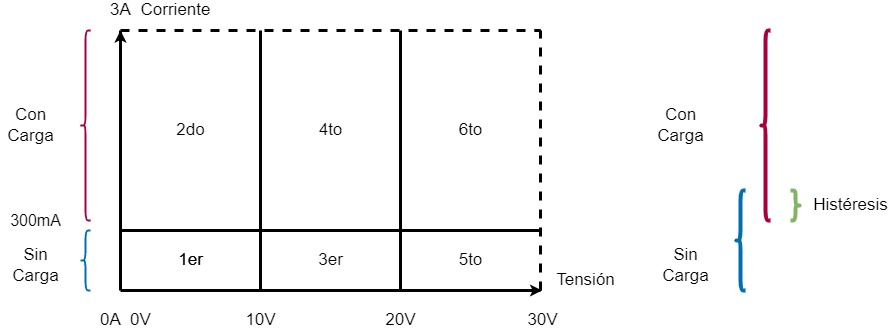
\includegraphics[scale=0.5]{./imagenes/matriz.jpg}
    \caption{Mapeo del rango de funcionamiento de la fuente.}
    \label{F:mapeo_cuadrantes}
\end{figure}\par

Un desafío de esta aproximación surge al acercarse a las zonas de transición entre las constantes del controlador, donde se produce un transitorio problemático en el cual el sistema podría perder estabilidad al cambiar de cuadrante. Para mitigar este inconveniente y asegurar que el controlador permanezca en el nuevo estado deseado, se desarrolló una ventana de histéresis como se ve en la parte derecha de la Figura \ref{F:mapeo_cuadrantes}. Esta ventana proporciona un amplio margen que garantiza que la transición se complete de manera correcta, manteniendo la estabilidad del sistema en todo momento.


\subsection{Soft Reset}
Para evitar la malinterpretación de las variables durante el funcionamiento, es importante mencionar la presencia de un \textit{soft reset} en el algoritmo de control. Este reinicio asegura que se restablezcan todas las variables clave, incluyendo el error acumulado y el efecto integrador, lo cual es crucial para evitar que los valores previos afecten negativamente el comportamiento del sistema en el nuevo estado. Al realizar el \textit{soft reset} permite que el sistema se reinicie desde un punto de referencia estable, que sería del reposo. Esto garantiza una respuesta adecuada y controlada ante las nuevas condiciones a las que puede estar sometida la fuente evitando escenarios indeseados.\par 

\subsection{Protección ante sobretensiones y falso contacto}
En sistemas electrónicos, es común que las cargas puedan tolerar un valor de alimentación inferior al diseñado durante unos pocos milisegundos, hasta que la tensión alcanza su valor nominal. Sin embargo, esta tolerancia no se extiende a las sobretensiones, ya que incluso una sobretensión de corta duración puede ser suficiente para dañar los componentes electrónicos de una carga. Por esta razón, la fuente de alimentación implementa un mecanismo de protección contra sobretensiones, que desconecta inmediatamente el relé de salida al detectar un valor de tensión superior al límite permitido.\par

Una vez que la sobretensión ha sido eliminada y la tensión de salida se ha estabilizado dentro de los límites predefinidos durante un tiempo determinado, el relé de salida se vuelve a habilitar, permitiendo el acoplamiento seguro de la carga. Esta función es particularmente útil en situaciones donde se produce un falso contacto, que puede generar picos de tensión y perturbaciones en la salida de la fuente. De este modo, se ofrece una protección adicional para la carga, garantizando su integridad ante escenarios potencialmente dañinos.\par
Este mecanismo de protección no solo previene daños permanentes en los dispositivos conectados, sino que también asegura una mayor durabilidad y fiabilidad del sistema en su conjunto, al minimizar los riesgos asociados con fluctuaciones de tensión imprevistas. \par
